%Empieza configuracion de capitulo
\setstretch{1.0}
\titleformat{\chapter}[block]{\Large\bfseries}{CHAPTER \Huge\thechapter\vspace{25 pt}}{0 pt}{\\\fontsize{26}{36}\selectfont}
\titlespacing{\chapter}{0 pt}{30 pt}{50 pt}[0 pt]
\titleformat{\section}{\Large\bfseries}{\thesection}{0 pt}{\hspace{30 pt}}
\titleformat{\subsection}{\large\bfseries}{\thesubsection}{0 pt}{\hspace{30 pt}}
\pagestyle{fancy}
\fancyhead[LO,LE]{\footnotesize\emph{\leftmark}}
\fancyhead[RO,RE]{\thepage}
\fancyfoot[CO,CE]{}
%Termina configuracion de capitulo

\chapter{System Architecture}
\setstretch{1.5} %Regresa el interlineado a 1.5

\normalsize
\noindent
In this chapter we will cover the architecture of the system, from a hardware
and software perspective. As well as the MPI implementation we are going to
use. There is a brief description of the benchmarks (with the fixes
implemented). In the end we present the description of the topology implemented

\section{Embedded System}
\noindent

As we described in the theoretical framework an embedded system is some
combination of computer hardware and software, either fixed in capability or
programmable, that is specifically designed for a particular function. We will
describe hardware of the development board as well as the software we are going
to use (operating system and firmware).

\subsection{Development Board} The platform we will use for our experiment is the
Intel \makeatletter @  Atom-TM Processor E3825. Their main characteristics are
described in (table~\ref{tab:4.1}).\cite{E3825}:

    \begin{center}
    \rowcolors{1}{gray}{white}
    \begin{tabular}{ | l | r |}
        \hline
        Processor Number & E3825  \\ \hline
        \# of cores & 2  \\ \hline
        \# of Thread & 2  \\ \hline
        Clock Speed & 1.3 GHz  \\ \hline
        L2 Cache & 1MB  \\ \hline
        Instruction Set & 64 bit  \\ \hline
    \end{tabular}
    \captionof{table}{Intel Atom Processor E3825
    Specifications} \label{tab:4.1}
    \end{center}

The commercial name of this platform is Minnow board Max.  figure~\ref{fig:4.1}
and  figure~\ref{fig:4.2} This is a development platform for both
professionals and makers. Minnow board Max is an open hardware platform. The
concept of ''open-source hardware'' or ''open hardware'' is not yet as well
known or widespread as the free software or open-source software concept.
However, it shares the same principles: anyone should be able to see the source
(the design documentation in case of hardware), study it, modify it and share
it.\cite{CERN}

\begin{figure}[H]
\centering
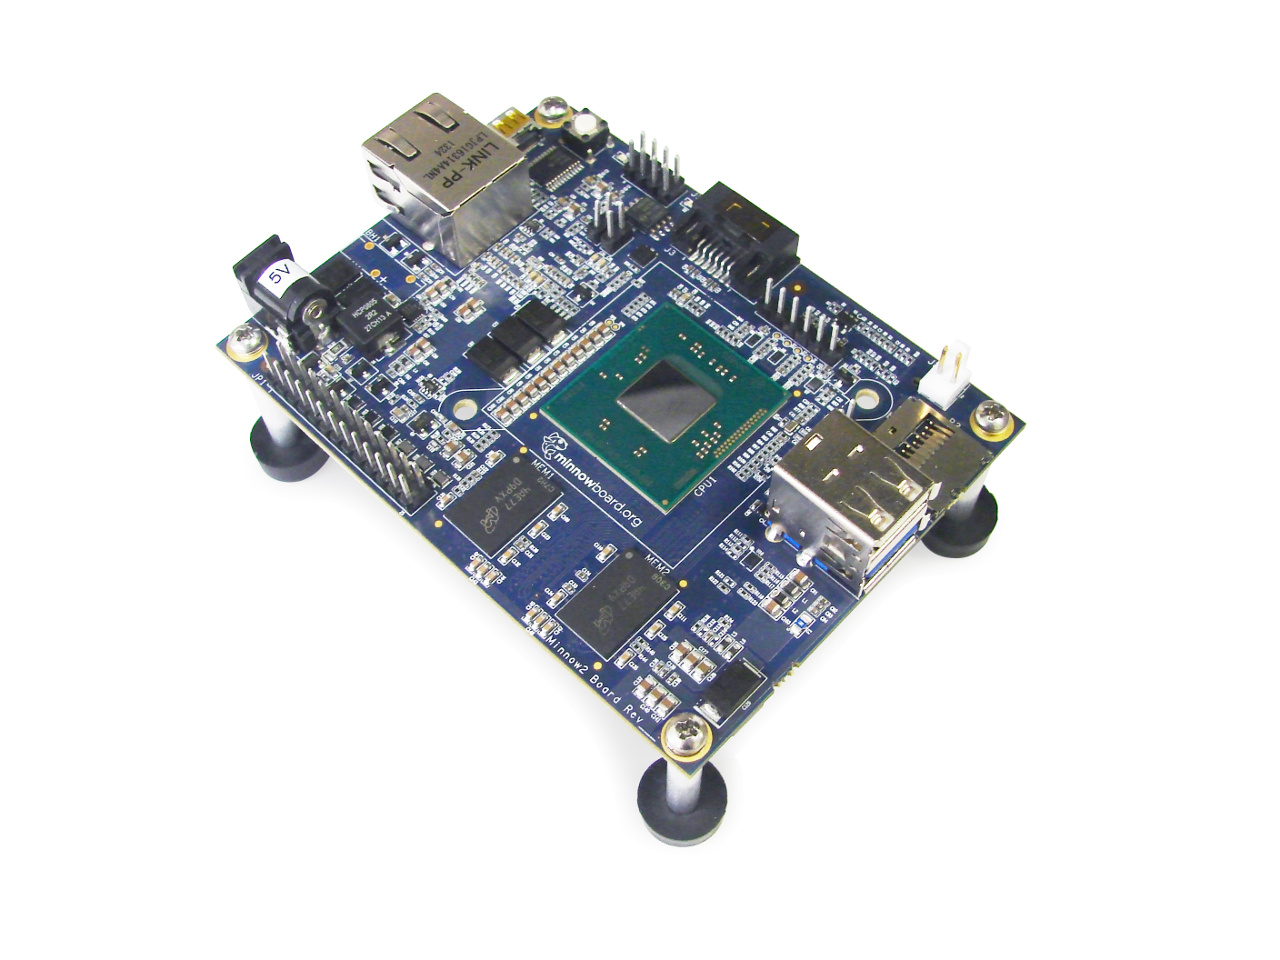
\includegraphics[width=0.75\textwidth]{images/minnow-max.jpg}.png
\caption{The Minnow board Max}
\label{fig:4.1}
\end{figure}


\begin{figure}[H]
\centering
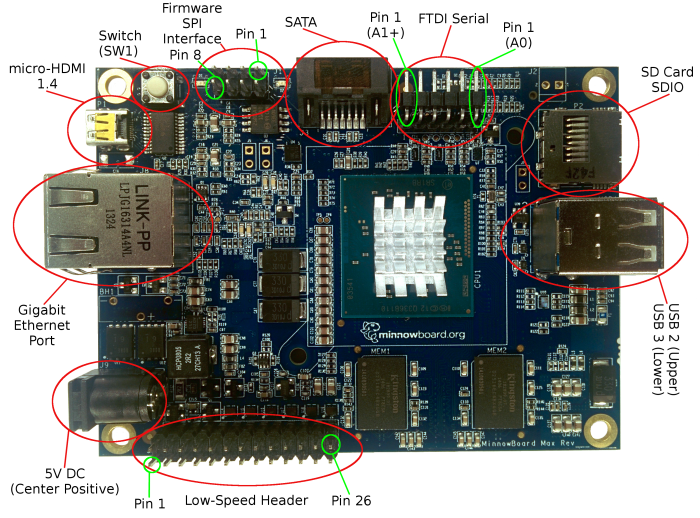
\includegraphics[width=0.75\textwidth]{images/minnow-max-2.png}
\caption{Connection Ports of the Minnow board Max}
\label{fig:4.2}
\end{figure}

\subsection{Embedded Operating System} 

Typical embedded system does not contain an operating system (ussually); but
due to the commplexity of current embedded applications is plenty necesary to
have an operating system that manage all the processes that current embedded
applications have. In order to perform the experiments we need a full Operating
System running on the development board. This means that it will require a boot
manager, a full file system , kernel and user space.  As we can see in
\cite{minnowboard} the board support multiple kind of Operating Systems. The OS
we are going to test are : 

\begin{itemize}
    \item Fedora project (Linux base) \cite{fedora}
    \item Clear Linux for Intel Architecture (Linux base) \cite{clear-linux}
    \item Yocto project (Linux base) \cite{yocto-project}
\end{itemize}

We will need to experiment which one is better for our needs. The reason why to
prove multiple  operating systems is because is necessary to find the best one.
There are multiple configurations inside each one that makes the performance of
the distributed system different. 

\subsection{Embedded Firmware}

The Minnow Board MAX platform is a low cost, commercially available, reference
platform for hardware, software and firmware developers who wish to work within
an open design development environment. Minnow Board MAX design specifications
and materials have been provided to the open community for the purpose of
enabling the community to experiment and develop technical solutions based upon
the Minnow Board MAX design.

The Minnow Board MAX firmware download page presents firmware components for the
Minnow Board MAX reference board. This firmware is provided to the community for
the purpose of enabling open development and experimentation. For this
experiment we have downloaded the official BIOS Firmware Binary Images
\cite{minnowmax-firmware}

\section{Topologies}

In computer networking, topology refers to the layout of connected devices. This
article introduces the standard topologies of networking

Think of a topology as a network's virtual shape or structure. This shape does
not necessarily correspond to the actual physical layout of the devices on the
network. For example, the computers on a home network may be arranged in a
circle in a family room, but it would be highly unlikely to find a ring
topology there.

Network topologies are categorized into the following basic types:

\begin{itemize}
    \item bus
    \item ring
    \item star
    \item tree
    \item mesh
\end{itemize}

More complex networks can be built as hybrids of two or more of the above basic
topologies.

For our experiments we will use the star topology (figure~\ref{fig:4.3}). In
local area networks with a star topology, each network host is connected to a
central hub with a point-to-point connection. So it can be said that every
computer is indirectly connected to every other node with the help of the hub.
In Star topology every node (computer workstation or any other peripheral) is
connected to a central node called hub, router or switch. The switch is the
server and the peripherals are the clients. The network does not necessarily
have to resemble a star to be classified as a star network, but all of the
nodes on the network must be connected to one central device. All traffic that
traverses the network passes through the central hub. The hub acts as a signal
repeater. The star topology is considered the easiest topology to design and
implement. An advantage of the star topology is the simplicity of adding
additional nodes. The primary disadvantage of the star topology is that the hub
represents a single point of failure.

\begin{figure}[H]
\centering
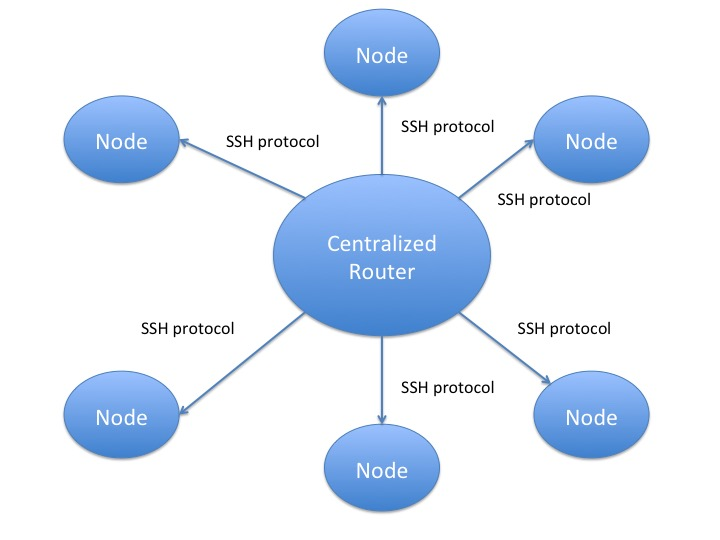
\includegraphics[width=0.75\textwidth]{images/star_topology.png}
\caption{Star topology diagram}
\label{fig:4.3}
\end{figure}


\section{Architecture Diagram}

After understanding all the parts of the system now we can describe the full
architecture of our experiments. The figure~\ref{fig:4.4} shows the diagram of
the final architecture in an star topology. As you can see the system can
increase the numbers of nodes (Minnow board platforms) if we want to increase
the compute capacity.


\begin{figure}[H]
\centering
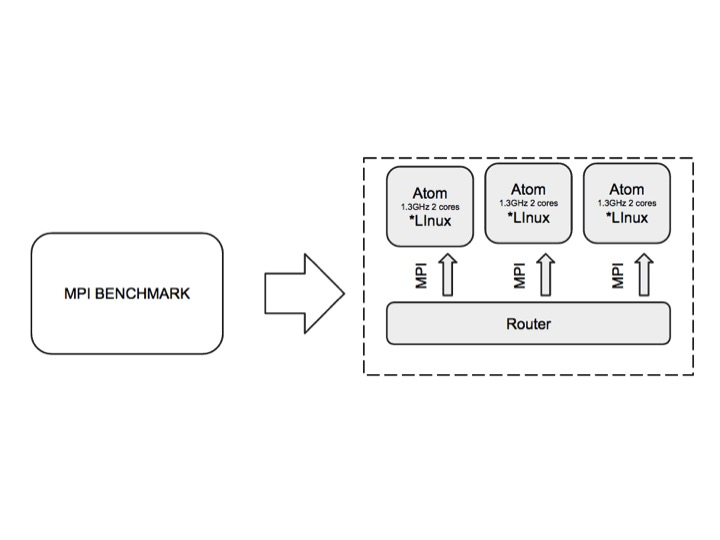
\includegraphics[width=0.75\textwidth]{images/full_diagram.jpg}
\caption{System Architecture Diagram }
\label{fig:4.4}
\end{figure}

\noindent

\clearpage
